\section{Rifrazione vetro}
L'ultima misurazione aveva come obiettivo quello di determinare l'indice di rifrazione del vetro; anche in questo caso è stato necessario contare il numero di frange passanti per un riferimento scelto, movimento delle quali causate da un componente aggiuntivo.

Tale componente, sul quale è montata una lastra di vetro, permette il cambiamento della figura di interferenza attraverso la rotazione della lastra stessa. Prima di iniziare l'esperimento è stato necessario determinare l'angolo di inversione, nel nostro caso $\theta = 0,2 \, ^\circ$, che determina il punto in cui le frange invertono il loro moto. 

Per una rotazione di $5 \, ^\circ$ abbiamo ricavato diversi $\Delta N$, riportati di seguito con il relativo istogramma:

\FloatBarrier
\begin{table}[h!]
    \centering
    \begin{tabular}{ccc}
    &\Delta N\\
    \hline
         & 23 & 24 \\
         & 23 & 24 \\
         & 22 & 21 \\ 
         & 25 & 25 \\
         & 23 & 23 \\
    \hline\hline
    \end{tabular}
    \caption{}
\end{table}
\begin{figure}[h!]
    \centering
    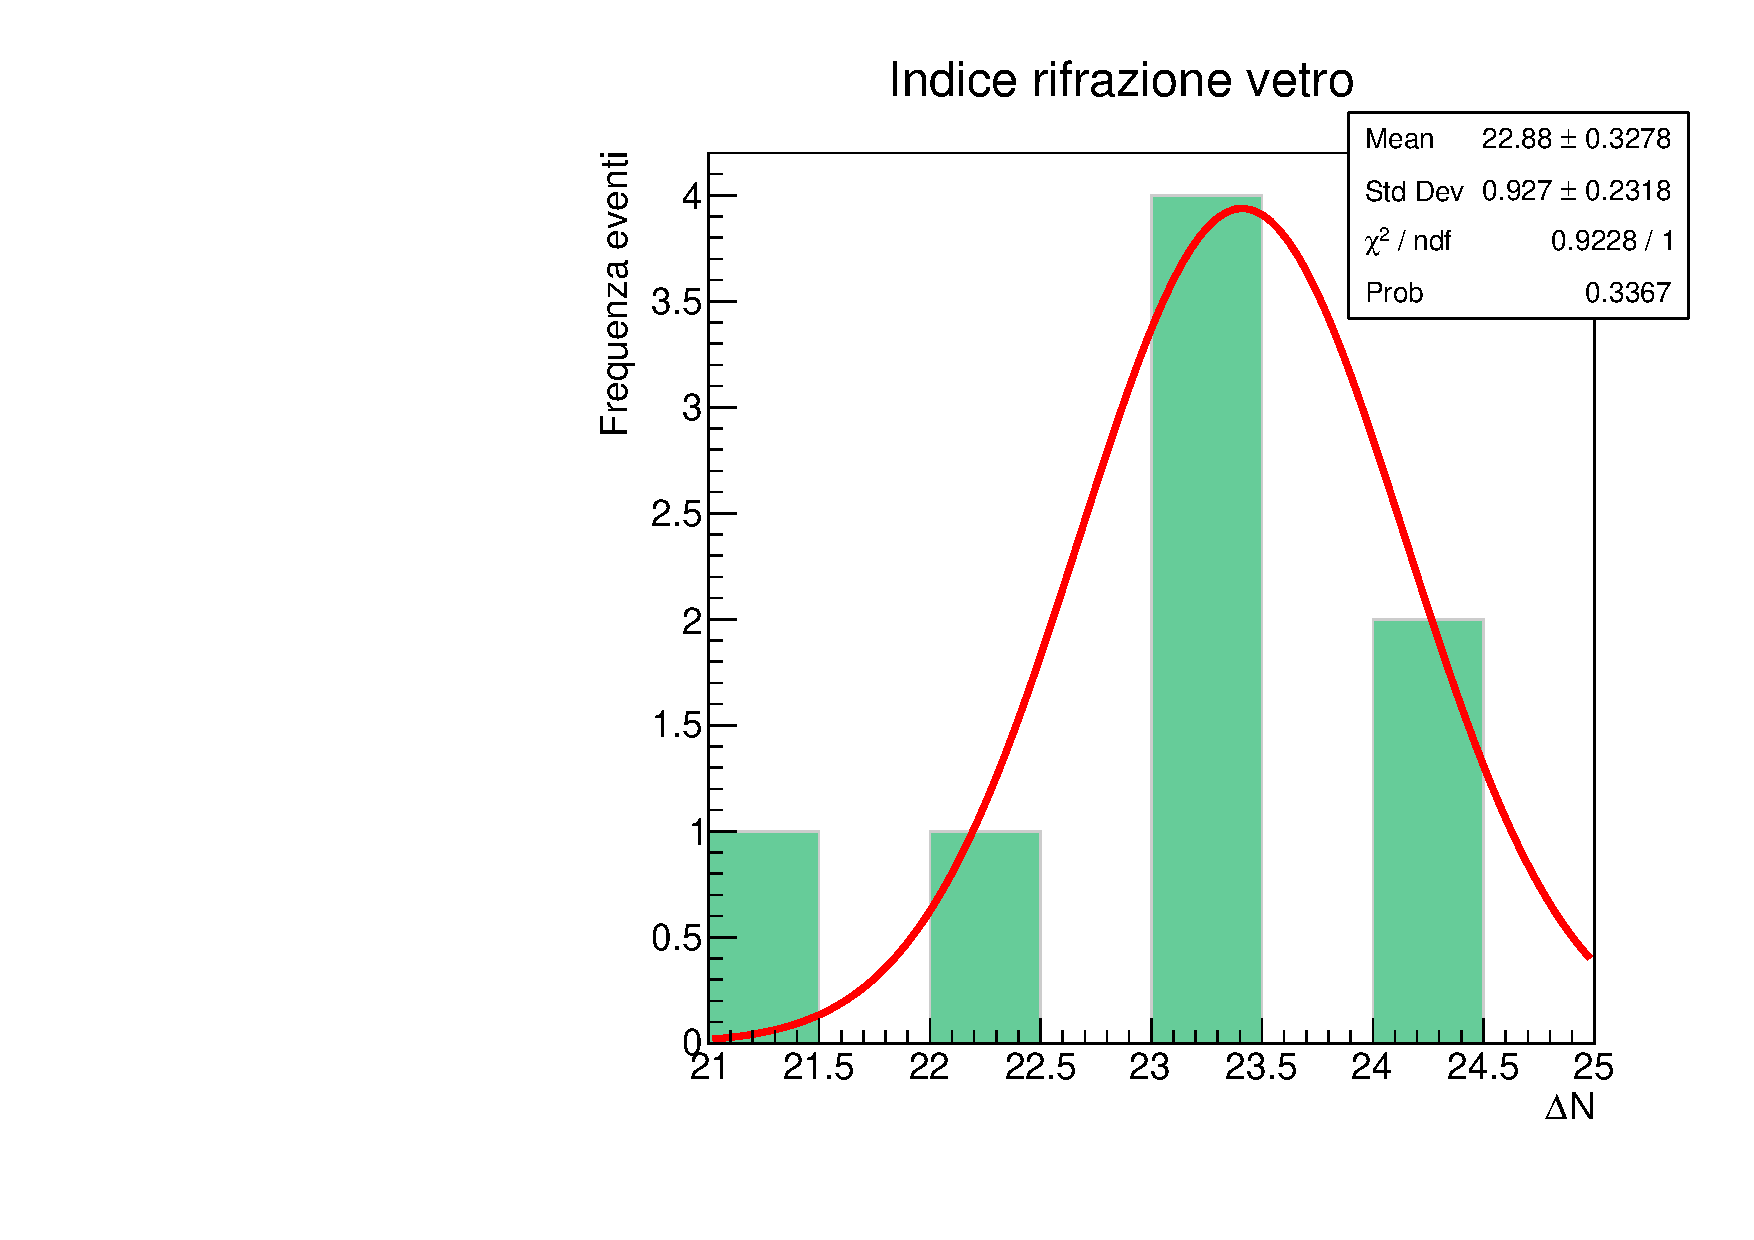
\includegraphics[scale=.4]{immagini/vetro.pdf}
    \caption{}
    \label{fit vetro}
\end{figure}
\FloatBarrier

Dopo aver ripetuto più volte la misura di \textit{d}, riportiamo i dati in tabella, abbiamo ricavato il valore medio di $d = 0,57\, \pm 0,006\, \operatorname{cm}$
\FloatBarrier
\begin{table}[h!]
    \centering
    \begin{tabular}{ccc}
    &\textit{d}\,(cm)\\
    \hline
         & 0.576 \\
         & 0.561 \\
         & 0.571 \\ 
         & 0.571 \\
         & 0.573 \\
    \hline\hline
    \end{tabular}
    \caption{}
\end{table}
\FloatBarrier
Utilizzando, quindi, il valore per \textit{d} trovato e le misure di $\Delta N$, attraverso l'Eq. \ref{eq 3}, abbiamo ricavato i seguenti valori

\FloatBarrier
\begin{table}[h!]
    \centering
    \begin{tabular}{ccc}
    &$n_{\text {vetro }}$ \\
    \hline
        & 1,495  & 1,528\\
        & 1,495  & 1,528\\
        & 1,464  & 1,433\\  
        & 1,563  & 1,563\\
        & 1,495  & 1,495\\
    \hline\hline
    \end{tabular}
    \caption{}
\end{table}
\FloatBarrier
\noindent
\begin{figure}[h!]
    \centering
    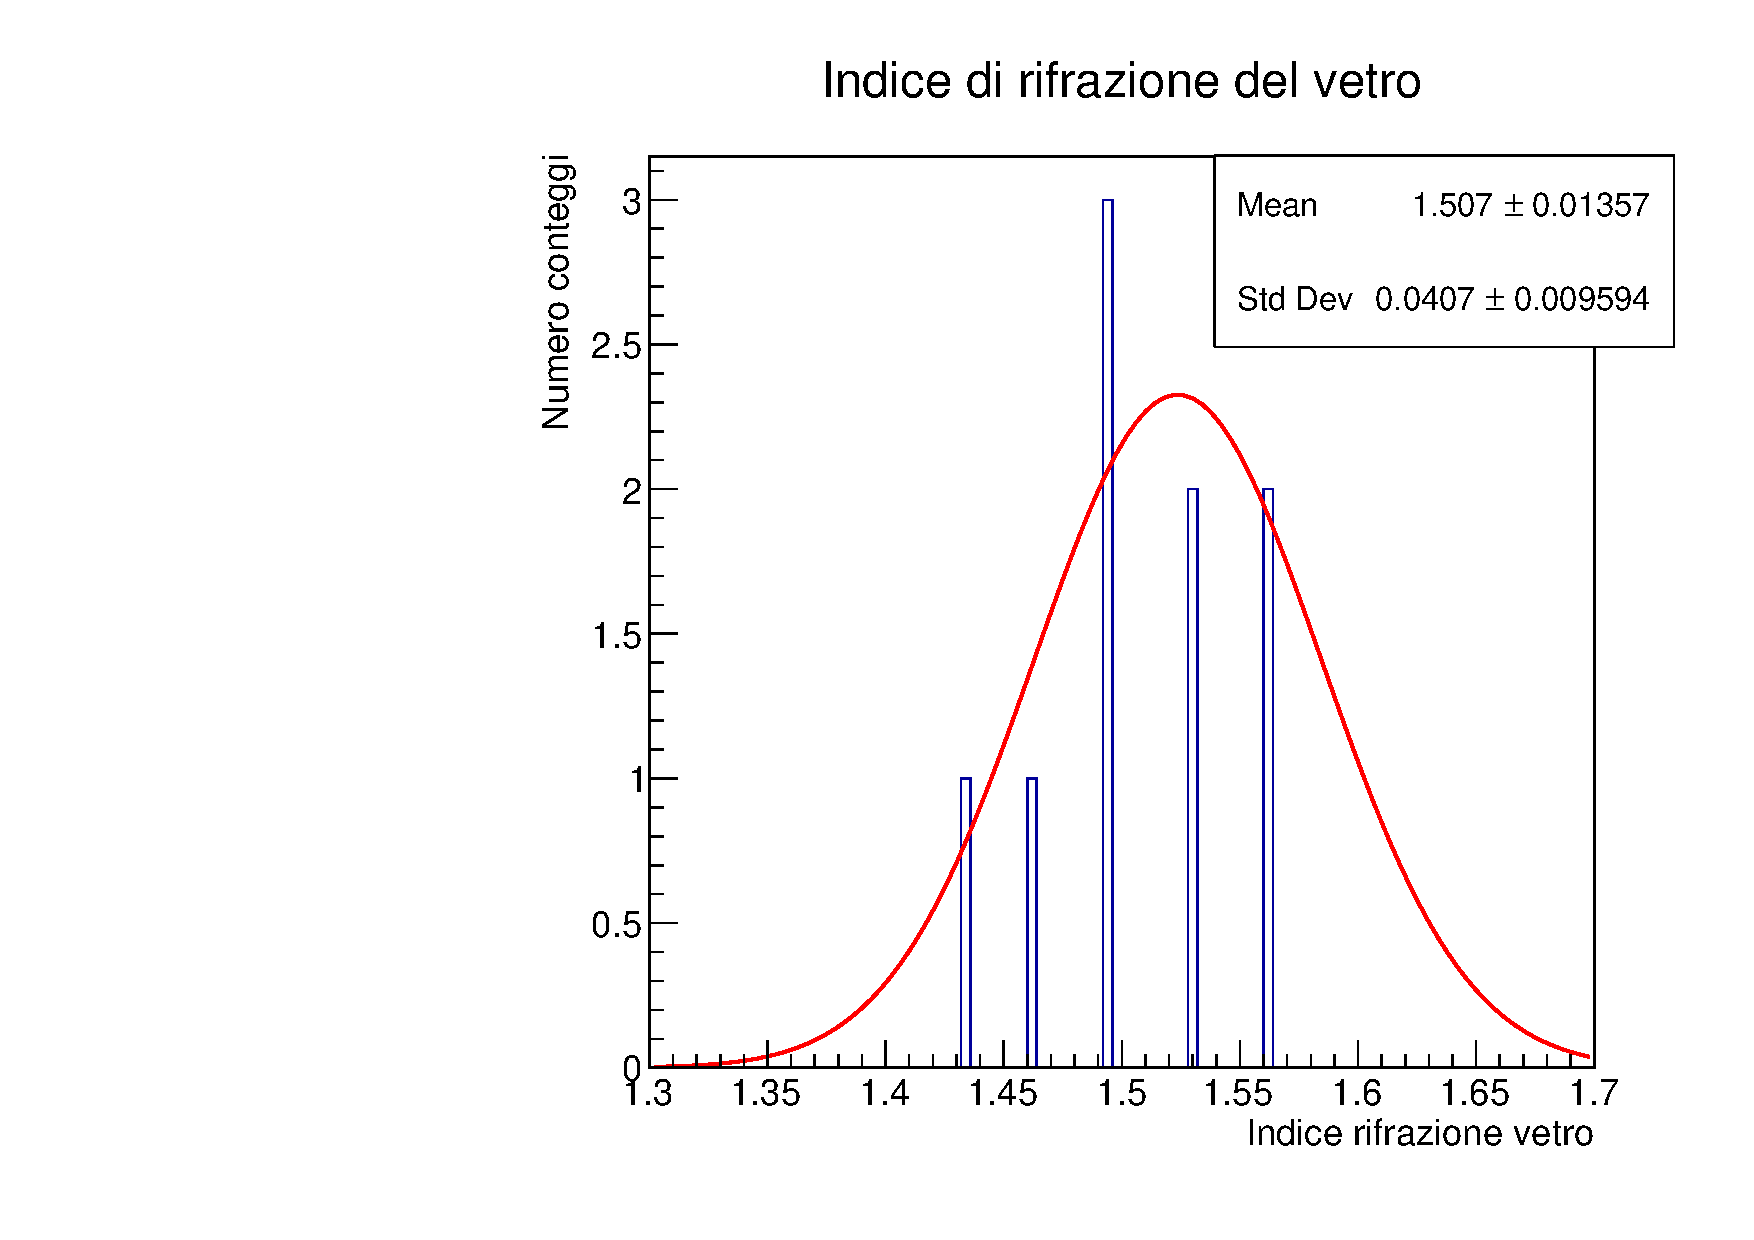
\includegraphics[scale=.4]{immagini/vetro copia.pdf}
    \caption{}
    \label{fig:my_label}
\end{figure}
Infine abbiamo dunque ottenuto il valore del coefficiente di rifrazione del vetro pari a 
$$
\eta_{\text{vetro}}=1,507\pm0,013
$$


